\chapter{youBot placing experiment}
\section{Deliverables 6.1}
\textbf{Run the complete experiment with a KUKA youBot arm, i.e. run all 180 experimental trials and perform any necessary preprocessing of the data. You should submit a written report covering your observations, including appropriate figures. Your report should include:}

\subsection{Description of the experiment}

\begin{itemize}
	\item We were provided with a small, a medium and a large object.
	\item Each object has to be grasped and moved into 3 positions: Left, Right and Straight. The grasping, movement and release was pre-programmed.
	\item Each object has to be moved into each position 20 times.
	\item The following steps were repeated each time the experiment had to be performed:
	\begin{itemize}
		\item 1) Place the object on the marker on the table.
		\item 2) Grab the object using the arm.
		\item 3) Move the object to one of the 3 positions using the arm.
	\end{itemize}
	\item The measurements were recorded in a file for each measurement. Each file contained 50 JSON objects which were separated by lines counting the measurements.
	\item In order to extract the poses from this a python program was written to create clean CSV files which contain only the poses.
	\item Sorting of the files is handled by a bash script.
\end{itemize}


\subsection{Any observations made during the execution that may help to understand the outcome of the experiments; for instance, are there any particular sources of error that may affect the results of the experiment?}

\begin{itemize}
	\item In order to minimize all external sources of error, we have closed the curtains and used artificial light provided by the lamps at the ceiling.
	\item Since we measured vibrations in the table whenever the arm was moving we have only taken our measurements when the arm was not moving
	\item We did not move the chaird or walk while performing measurements since we were able to detect vibrations because of movement in the room
\end{itemize}

\subsection{A description of the pose filtering procedure you used and any observations that you may have made during the filtering process (e.g. on average, how many outliers are there per single experimental trial)}

\begin{itemize}
	\item For each run of the experiment a measurement was taken using the optical tracker.
	\item Each measurement recording consists of 50 pose recordings. This measurement redundancy is added to avoid measurement faults. The average of the 50 poses is taken as final pose for each measurement.
	
\end{itemize}


\subsection{The saved preprocessed data as Excel or LibreOffice Calc file or in a similar machine-readable form}

Those recordings have been saved in CSV files for each of the 3 experiments. They can be found in: \texttt{recordings/CSVs}.

\subsection{A visualization of the obtained final object poses. You are free to use any suitable visual representation for the data (using what you have already learned during the LEGO experiment). Hint: Given the different object-place combinations in the experiment, think about what we might want to illustrate with the visualization (e.g. the distribution of poses per object? the distribution of poses per motion direction? the distribution of all poses?)}


\begin{figure}[ht!]
	\centering
	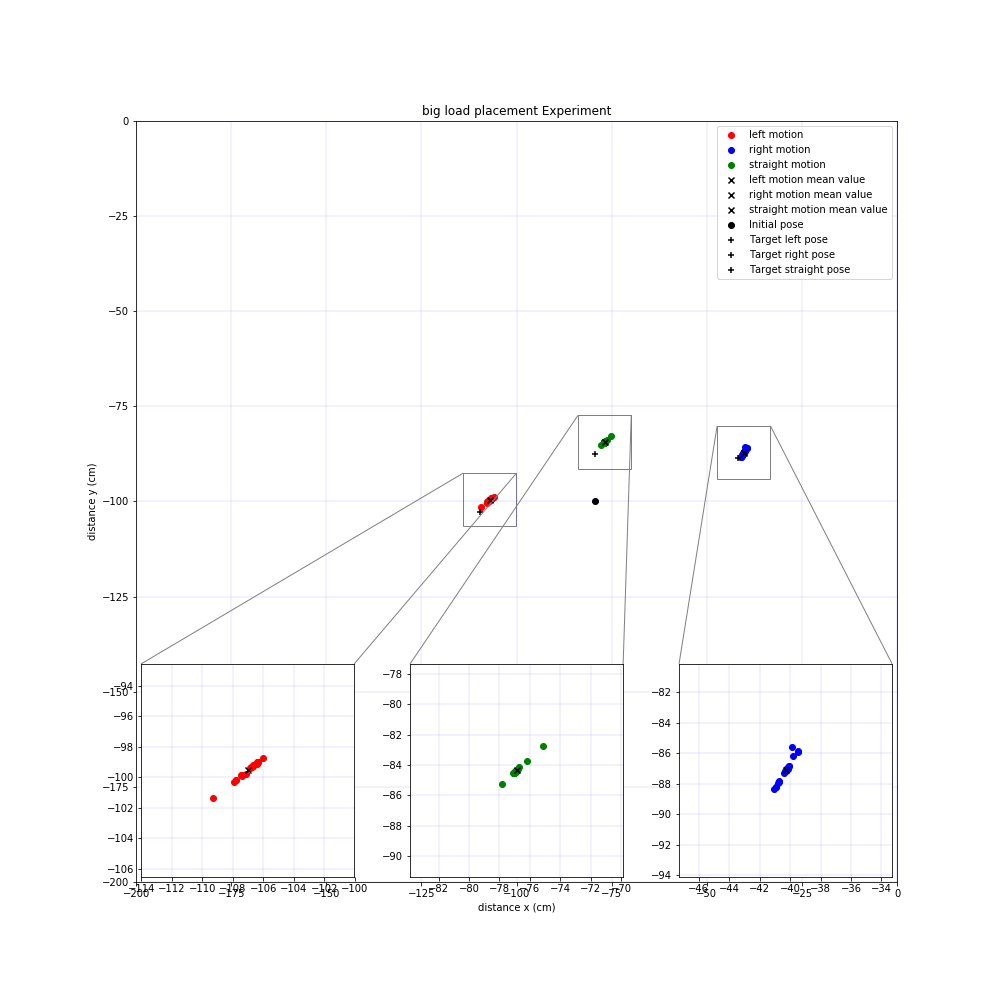
\includegraphics[width=0.6\linewidth]{images/big}
	\caption{Results of the Big Load Placement Experiment}
	\label{fig:big}
\end{figure}
\begin{figure}[ht!]
	\centering
	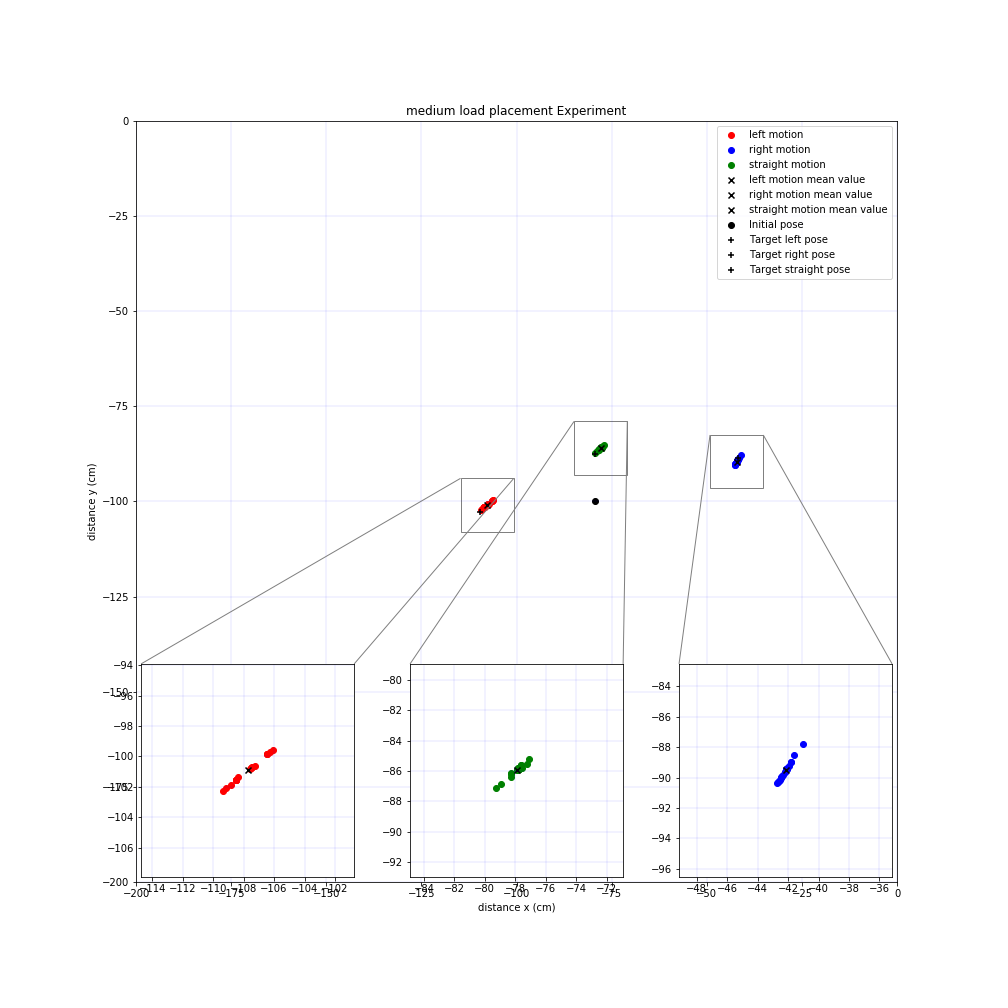
\includegraphics[width=0.6\linewidth]{images/medium}
	\caption{Results of the Medium Load Placement Experiment}
	\label{fig:medium}
\end{figure}
\begin{figure}[ht!]
	\centering
	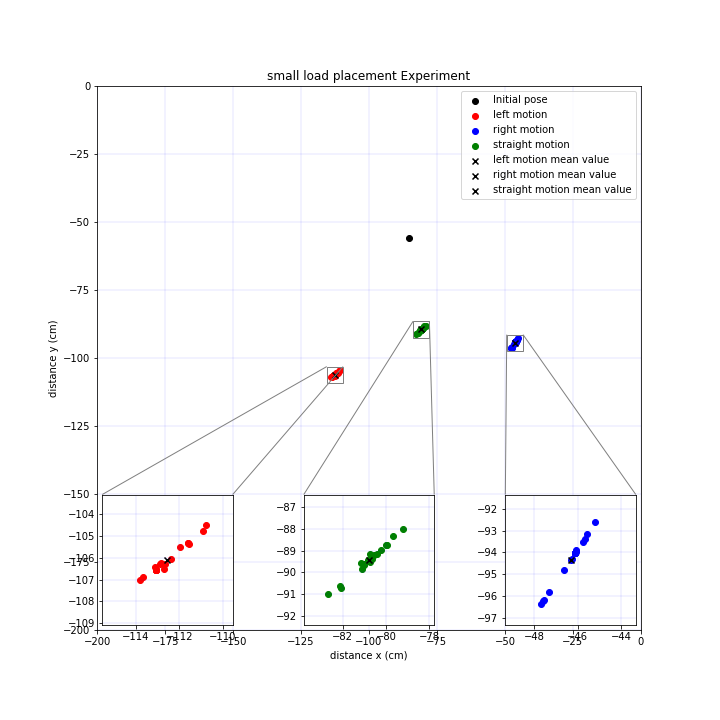
\includegraphics[width=0.6\linewidth]{images/small}
	\caption{Results of the Small Load Placement Experiment}
	\label{fig:small}
\end{figure}



\begin{figure}[ht!]
	\centering
	\begin{subfigure}[b]{0.3\textwidth}
		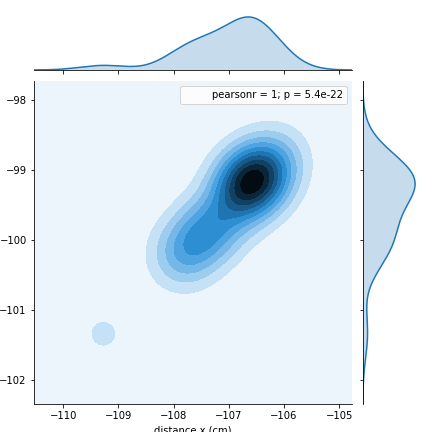
\includegraphics[width=\textwidth]{images/big_left.png}
		\caption{Left motion final pose.}
		\label{distribution-right-turn}
	\end{subfigure}
	\qquad
	\begin{subfigure}[b]{0.3\textwidth}
		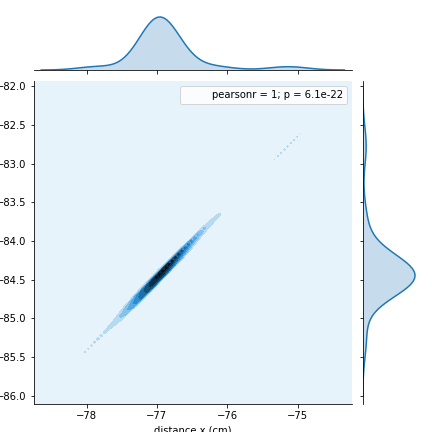
\includegraphics[width=\textwidth]{images/big_straight.png}
		\caption{Straight motion final pose.}
		\label{distribution-right-turn}
	\end{subfigure}
	\qquad
	\begin{subfigure}[b]{0.3\textwidth}
		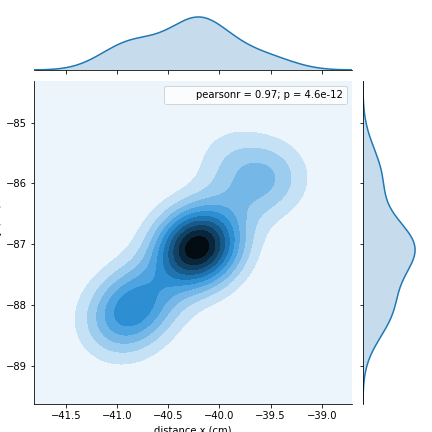
\includegraphics[width=\textwidth]{images/big_right.png}
		\caption{Right motion final pose.}
		\label{distribution-straight-motion}
	\end{subfigure}
	\caption{Gaussian and marginal distributions Final pose distribution - Big object}
\end{figure}

\begin{figure}[ht!]
	\centering
	\begin{subfigure}[b]{0.3\textwidth}
		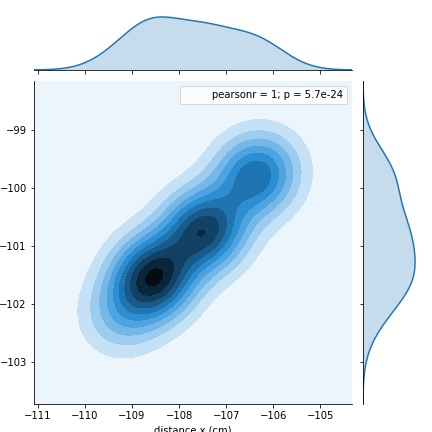
\includegraphics[width=\textwidth]{images/medium_left.png}
		\caption{Left motion final pose.}
		\label{distribution-right-turn}
	\end{subfigure}
	\qquad
	\begin{subfigure}[b]{0.3\textwidth}
		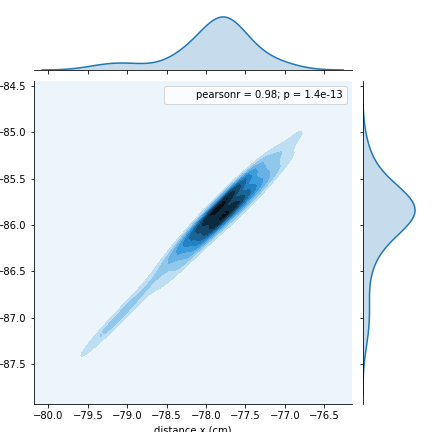
\includegraphics[width=\textwidth]{images/medium_straight.png}
		\caption{Straight motion final pose.}
		\label{distribution-right-turn}
	\end{subfigure}
	\qquad
	\begin{subfigure}[b]{0.3\textwidth}
		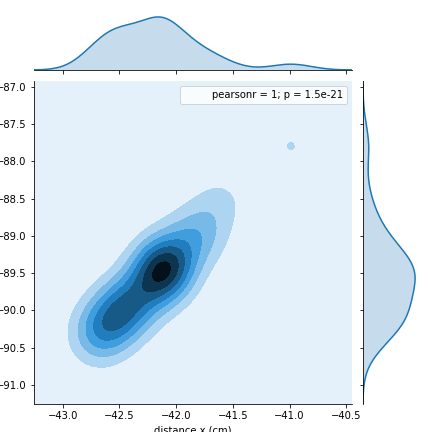
\includegraphics[width=\textwidth]{images/medium_right.png}
		\caption{Right motion final pose.}
		\label{distribution-straight-motion}
	\end{subfigure}
	\caption{Gaussian and marginal distributions Final pose distribution - Medium object}
\end{figure}

\begin{figure}[ht!]
	\centering
	\begin{subfigure}[b]{0.3\textwidth}
		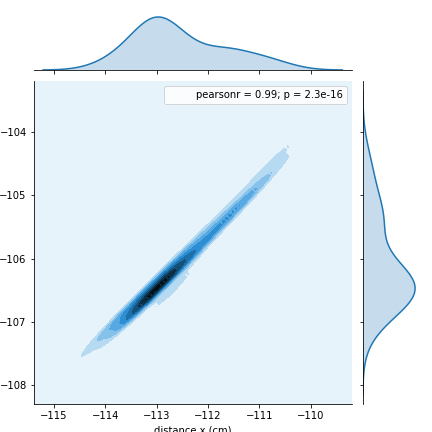
\includegraphics[width=\textwidth]{images/small_left.png}
		\caption{Left motion final pose.}
		\label{distribution-right-turn}
	\end{subfigure}
	\qquad
	\begin{subfigure}[b]{0.3\textwidth}
		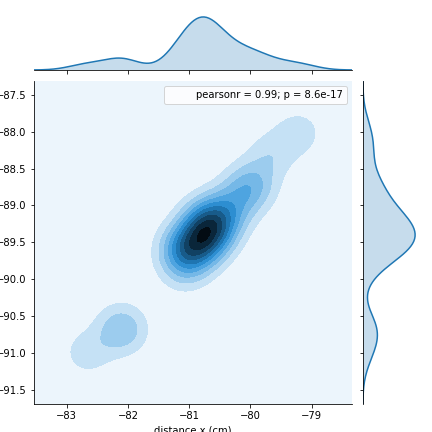
\includegraphics[width=\textwidth]{images/small_straight.png}
		\caption{Straight motion final pose.}
		\label{distribution-right-turn}
	\end{subfigure}
	\qquad
	\begin{subfigure}[b]{0.3\textwidth}
		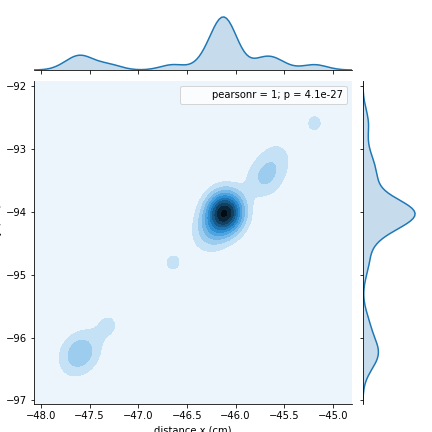
\includegraphics[width=\textwidth]{images/small_right.png}
		\caption{Right motion final pose.}
		\label{distribution-straight-motion}
	\end{subfigure}
	\caption{Gaussian and marginal distributions Final pose distribution - Small object}
\end{figure}


%%%%%%%%%%%%%%%%%%%%%%%%%%%%%%%%%%%%%%%%%%%%%%%%%%%%%%%%%%%%%%%%%%%%%%%%%%%%%